\chapter{Pendahuluan}
\label{chap:pendahuluan}

\section{Latar Belakang}
\label{sec:latar_belakang}
KIRI\cite{kiritravel} (Gambar \ref{fig:1_kiritravel}) merupakan situs web untuk membantu pengguna menemukan rute transportasi umum ke tempat tujuannya. Dengan memasukkan lokasi awal serta lokasi tujuan pengguna tersebut, situs web KIRI akan memberikan langkah-langkah (contoh: berjalan sejauh berapa meter, menggunakan angkot, dan sebagainya) tercepat untuk sampai ke lokasi tujuan.

\begin{figure}[htbp]
	\centering
		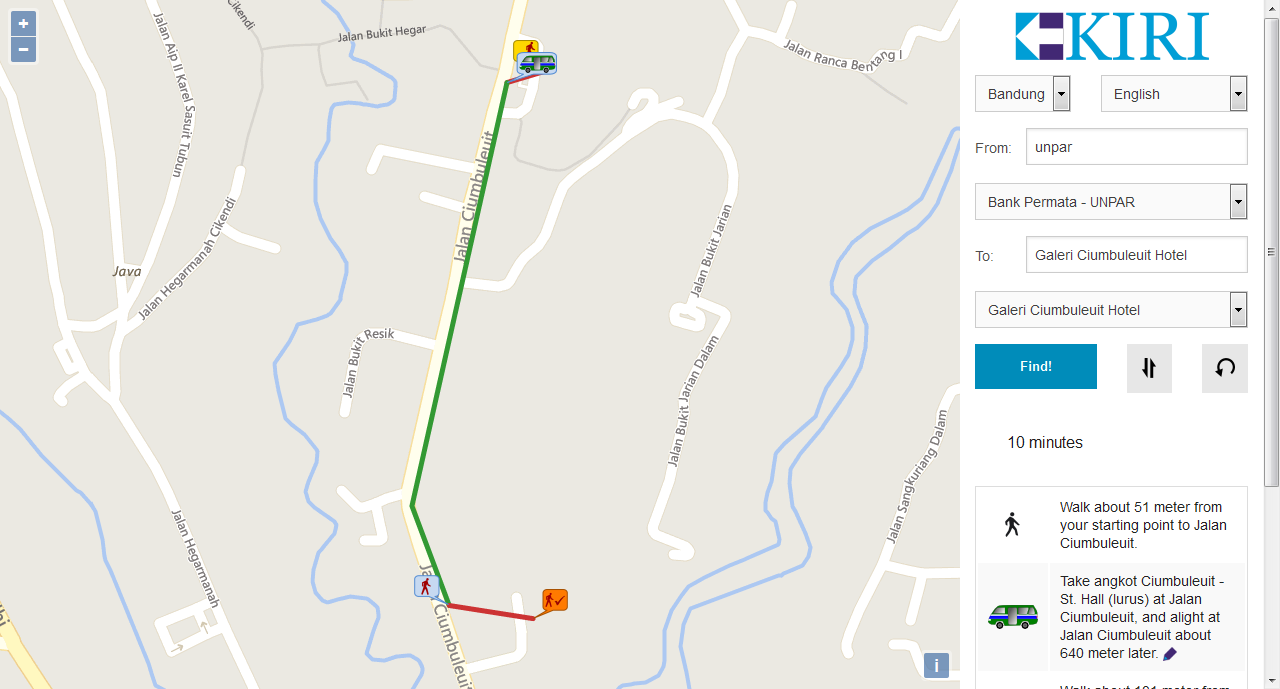
\includegraphics[scale=0.35]{Gambar/1_kiritravel.png}
	\caption{Situs web KIRI\cite{kiritravel}}
	\label{fig:1_kiritravel}
\end{figure}

KIRI \textit{Dashboard}\cite{devkiritravel} (Gambar \ref{fig:1_kiridashboard}) adalah bagian dari situs web KIRI. KIRI \textit{Dashboard} berfungsi sebagai pengatur proses CRUD (\textit{Create, Read, Update,} dan \textit{Delete}) daftar rute yang terdapat dalam \textit{database} situs web KIRI. KIRI \textit{Dashboard Server Side} menggunakan bahasa PHP dalam pembuatannya\cite{kiridashboard}. Bahasa PHP kurang cocok untuk proyek skala besar seperti \textit{dashboard}. Salah satu penyebab bahasa PHP kurang cocok adalah karena tidak ada deklarasi dan tipe variabel dalam penggunaan bahasa PHP.

Java merupakan bahasa pemrograman yang umum digunakan oleh banyak orang. Selain umum digunakan, Java juga merupakan bahasa pemrograman yang lebih terstruktur dibandingkan dengan PHP. Adanya deklarasi dan tipe variabel pada Java membuat setiap variabel memiliki kegunaan yang lebih jelas dan mudah dimengerti. Play Framework merupakan salah satu \textit{framework} yang membantu implementasi Java dalam pembuatan suatu situs web. Play Framework juga cocok untuk proyek skala besar karena arsitekturnya sudah menggunakan konsep MVC (\textit{Model View Controller})\cite{playforjava}.

\begin{figure}[htbp]
	\centering
		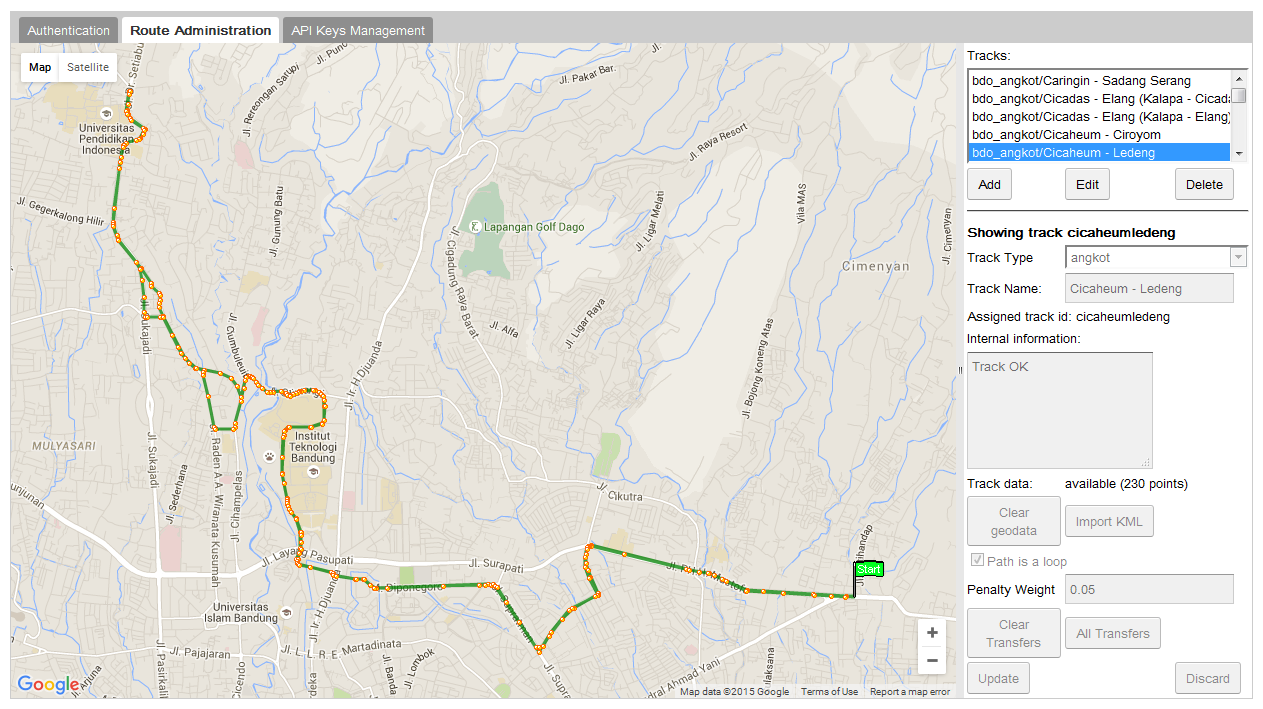
\includegraphics[scale=0.35]{Gambar/1_kiridashboard.png}
	\caption{KIRI \textit{Dashboard}\cite{devkiritravel}}
	\label{fig:1_kiridashboard}
\end{figure}

Berdasarkan ditemukannya kekurangan-kekurangan pada KIRI \textit{Dashboard Server Side} seperti yang telah dijelaskan, maka solusi untuk mengatasi kekurangan tersebut adalah dibuatlah penelitian ini untuk mengubah KIRI \textit{Dashboard Server Side} yang semula dalam bahasa PHP menjadi bahasa Java dengan menggunakan Play Framework.

\section{Rumusan Masalah}
\label{sec:rumusan_masalah}
Berikut adalah susunan permasalahan yang akan dibahas pada penelitian ini:
	\begin{enumerate}
		\item Bagaimana isi kode KIRI \textit{Dashboard Server Side} dan apa saja kekurangan yang ada di dalamnya?
		\item Bagaimana cara kerja Play Framework berbasis MVC?
		\item Bagaimana melakukan \textit{porting} KIRI \textit{Dashboard Server Side} yang semula dalam bahasa PHP menjadi bahasa
Java dengan menggunakan Play Framework?
	\end{enumerate}
	
\section{Tujuan}
\label{sec:tujuan}
Berdasarkan rumusan masalah yang telah dibuat, maka tujuan penelitian ini dijelaskan ke dalam poin-poin sebagai berikut:
	\begin{enumerate}
		\item Mengetahui isi kode KIRI \textit{Dashboard Server Side} dan kekurangan-kekurangan yang ada di dalamnya.
		\item Mengetahui cara kerja Play Framework berbasis MVC.
		\item Melakukan \textit{porting} KIRI \textit{Dashboard Server Side} yang semula dalam bahasa PHP menjadi bahasa
Java dengan menggunakan Play Framework.
	\end{enumerate}
	
\section{Batasan Masalah}
\label{sec:batasan_masalah}
Penelitian ini dibuat berdasarkan batasan-batasan sebagai berikut:
	\begin{enumerate}
		\item Play Framework yang digunakan selama penelitian ini adalah versi 2.4.3.
		\item \textit{Porting} Kode KIRI \textit{Dashboard Server Side} yang dilakukan adalah berdasarkan versi terbaru dari Github dengan \textit{username}: ``pascalalfadian''\cite{kiridashboard}.
	\end{enumerate}
	
\section{Metode Penelitian}
\label{sec:metode_penelitian}
Berikut adalah metode penelitian yang digunakan dalam penelitian ini:
	\begin{enumerate}
		\item Melakukan studi literatur mengenai kode KIRI \textit{Dashboard Server Side}, MySQL Spatial Extensions, dan Play Framework.
		\item Menganalisis teori-teori untuk membangun KIRI \textit{Dashboard Server Side} dalam bahasa Java dengan menggunakan Play Framework.
		\item Merancang KIRI \textit{Dashboard Server Side} dalam bahasa Java dengan menggunakan Play Framework.
		\item Melakukan \textit{porting} kode situs web KIRI \textit{Dashboard Server Side} menjadi Java dengan menggunakan Play Framework.
		\item Melakukan pengujian terhadap fitur-fitur yang sudah dibuat.
	\end{enumerate}

\section{Sistematika Penulisan}
\label{sec:sistematika_penulisan}
Setiap bab dalam penelitian ini memiliki sistematika penulisan yang dijelaskan ke dalam poin-poin sebagai berikut:
	\begin{enumerate}
		\item Bab 1: Pendahuluan, yaitu membahas mengenai gambaran umum penelitian ini. Berisi tentang latar belakang, rumusan masalah, tujuan, batasan masalah, metode penelitian, dan sistematika penulisan.
		\item Bab 2: Dasar Teori, yaitu membahas mengenai teori-teori yang mendukung berjalannya penulisan ini. Berisi tentang MySQL Spatial Extensions dan Play Framework.
		\item Bab 3: Analisis, yaitu membahas mengenai analisa masalah. Berisi tentang analisis kode KIRI \textit{Dashboard Server Side} dan analisis kekurangan-kekurangan kode KIRI \textit{Dashboard Server Side}.
		\item Bab 4: Perancangan, yaitu membahas mengenai perancangan yang dilakukan sebelum melakukan tahapan implementasi. Berisi tentang perancangan fitur CRUD KIRI \textit{Dashboard Server Side} menggunakan Play Framework, perancangan basis data, dan perancangan antarmuka KIRI \textit{Dashboard} menggunakan Play Framework.
		\item Bab 5: Implementasi dan Pengujian, yaitu membahas mengenai implementasi dan pengujian aplikasi yang telah dilakukan. Berisi tentang implementasi dan hasil pengujian aplikasi.
		\item Bab 6: Kesimpulan dan Saran, yaitu membahas hasil kesimpulan dari keseluruhan penelitian ini dan saran-saran yang dapat
diberikan untuk penelitian berikutnya. Berisi tentang kesimpulan dan saran.
	\end{enumerate}